\documentclass[11pt]{article}

\usepackage[margin=1in]{geometry}
\usepackage{graphicx}
\usepackage{booktabs}
\usepackage{longtable}
\usepackage{float}
\usepackage[table]{xcolor}
\usepackage{microtype}
\usepackage{hyperref}
\usepackage{enumitem}
\usepackage{siunitx}
\usepackage{amsmath}
\usepackage{setspace}
\usepackage[numbers]{natbib}

\hypersetup{hidelinks}
\setlength{\parskip}{0.35em}
\setlength{\parindent}{0pt}
\setstretch{1.05}
\sisetup{group-separator={,}, group-minimum-digits=4}

\title{The Memory Wall: Data Structures vs. Hardware Reality \\
\large A Comprehensive Design-and-Measurement Record}
\author{Sheikh Mohsin}
\date{April 2026}

\begin{document}
\maketitle

\begin{abstract}
This manuscript documents the full design, implementation, and measurement rationale for the \textit{Performance-and-Data-Representation} project. The core objective is to show that algorithmic complexity alone is insufficient to predict performance on modern hardware, where memory latency dominates. We instrument sixteen data structures and gather high-density performance telemetry using hardware counters. This paper records every major decision---from counter selection and warmup policy to data layout perturbations---and links those choices to the empirical results. The end product is a reproducible, hardware-grounded narrative that explains why contiguity, locality, and cache-aware layouts consistently outperform pointer-heavy structures once datasets exceed cache capacity. The methodology follows principles articulated in Drepper's seminal memory-hierarchy analysis \citep{drepper2007}, with decisions tailored to the exact tooling and scripts present in this repository.
\end{abstract}

\tableofcontents
\clearpage

\section{Introduction}
Modern CPUs execute billions of instructions per second, yet a single trip to DRAM still costs on the order of hundreds of cycles. This disparity is the ``memory wall'' that throttles performance for many real-world data structures. In this project, we reject the assumption that asymptotic complexity alone predicts runtime. We instead measure data-structure performance under realistic, hardware-constrained conditions, focusing on locality and memory access behavior. 

The purpose of this manuscript is twofold: (1) to provide a rigorous technical record of the benchmark suite, and (2) to document every design decision and its rationale. The resulting system is not a toy benchmark but a reproducible measurement pipeline with detailed instrumentation, controlled variability, and a large empirical dataset (6,641 samples and 722.2B element traversals, per the included dataset and figures).

\section{Problem Statement and Research Questions}
The project explores a set of tightly scoped research questions:
\begin{enumerate}[label=\textbf{Q\arabic*}.]
    \item How does memory layout influence throughput for data structures that share similar algorithmic complexity?
    \item At what dataset sizes do cache boundaries become the dominant driver of performance collapse?
    \item Which hardware counters most clearly reflect the transition from compute-bound to memory-bound behavior?
    \item How do cache-aware and cache-oblivious layouts compare when measured on the same hardware and dataset sizes?
\end{enumerate}

These questions are addressed through controlled instrumentation and a structured parameter sweep that spans five orders of magnitude in problem size (\(10^3\) to \(10^8\)).

\section{Background and Related Work}
\subsection{The Memory Wall}
The memory wall describes the growing disparity between CPU speed and memory latency. While core clock rates and out-of-order execution reduce compute time, DRAM access latency remains high and comparatively stagnant. Drepper's comprehensive treatment of memory hierarchy \citep{drepper2007} emphasizes that effective performance is governed by how well data reuse and locality exploit caches. This manuscript adopts that viewpoint and uses memory behavior, not just operation counts, as the primary performance driver.

\subsection{Locality and Access Patterns}
Two classical locality principles guide the project:
\begin{itemize}
    \item \textbf{Spatial locality}: contiguous data is more likely to share cache lines.
    \item \textbf{Temporal locality}: recently accessed data is likely to be used again soon.
\end{itemize}
Data structures that store elements contiguously (arrays, vectors, or cache-line-packed nodes) benefit disproportionately from spatial locality and hardware prefetching. Pointer-heavy structures cause unpredictable loads that defeat prefetchers, serializing the pipeline and amplifying latency penalties.

\subsection{Hardware-Aware Algorithms}
The project's design is motivated by work in hardware-aware data structures and systems performance measurement \citep{patterson2017}. The benchmark suite isolates memory behavior and quantifies its performance cost, yielding a dataset suitable for both qualitative analysis and more formal modeling.

\section{Project Scope and Data Structures}
Sixteen data structures are implemented in C, each with a consistent measurement harness and data-generation policy. They are grouped into three families based on memory layout characteristics:\\

\textbf{Contiguous:} Array, Vector, Array-of-Structs (AoS), Struct-of-Arrays (SoA), Circular Buffer, Heap.\\
\textbf{Pointer-Chasing:} Linked List, Binary Search Tree (BST), Red-Black Tree, Skip List, Trie.\\
\textbf{Cache-Aware:} B-Tree, van Emde Boas Tree (vEB), Slab List, Hash Map, Deque.\\

The grouping is a deliberate explanatory device. It frames locality as the independent variable and allows results to be compared across families with similar algorithmic complexity but different layout strategies.

\section{Instrumentation Architecture}
\subsection{Counter Selection and Access}
Hardware counters are accessed using \texttt{perf\_event\_open} via \texttt{perf\_helper.h}. The following counters are enabled:
\begin{itemize}
    \item CPU cycles
    \item Instructions retired
    \item Cache misses (last-level)
    \item Branch instructions and branch misses
    \item L1 data-cache misses
    \item Data TLB misses
\end{itemize}
These counters allow computation of IPC, cache miss rates, and indicators of pipeline stalls. The selection emphasizes metrics that correlate with memory latency rather than pure compute throughput. Drepper notes that cache misses and TLB behavior often dominate runtime variance \citep{drepper2007}, which directly informs the decision to include both L1 and DTLB misses.

\subsection{Sampling and Aggregation}
Each benchmark run produces multiple samples per \(N\). A warmup phase (three passes over the data structure) primes the cache and branch predictor. Measurement samples are collected in a ``drowning loop'' that walks the structure and updates a volatile accumulator to prevent dead-code elimination. 

For each set of samples, the system computes:
\begin{itemize}
    \item median cycles
    \item minimum cycles
    \item coefficient of variation (CV\%)
    \item 95\% confidence interval half-width (using Bessel-corrected standard deviation)
\end{itemize}
The median is chosen for robustness against outliers, a decision consistent with the high-variance nature of hardware counters in noisy environments. The CV provides a fast diagnostic for unstable measurements, and CI values are reported for later downstream analysis.

\section{Data Layout Control: The Memory Shake}
The project uses an explicit ``memory shake'' to remove allocator-induced locality from pointer-based data structures. As shown in \texttt{linked\_list.c}, nodes are allocated sequentially, stored in a temporary array, and then randomly shuffled using a Fisher-Yates pass before linking. This creates an intentionally adverse layout, ensuring that the linked structure measures true pointer-chasing behavior rather than a benign sequential allocation artifact.

This choice was critical because malloc often returns contiguous addresses for sequential allocations. Without the shuffle, a linked list can exhibit misleading locality and distort the comparison against contiguous structures. The shuffle is therefore a necessary precondition for meaningful pointer-based measurements.

\section{Benchmark Harness and Sweep Strategy}
\subsection{Scale Ranges and Step Sizes}
The sweep strategy is implemented in \texttt{runperf.sh}. The system traverses five decades of \(N\) with a fixed step per decade:
\begin{itemize}
    \item 1,000--10,000, step 30
    \item 10,000--100,000, step 300
    \item 100,000--1,000,000, step 3,300
    \item 1,000,000--10,000,000, step 33,000
    \item 10,000,000--100,000,000, step 330,000
\end{itemize}
Each step is jittered per data structure to avoid repeated alignment with specific cache boundaries, and data structures are shuffled between each \(N\) slice to minimize thermal or time-correlated bias.

\subsection{Run Counts and Noise Control}
Run counts are adaptive to \(N\): tiny datasets run many iterations to reduce noise, while large datasets run fewer iterations to keep total runtime feasible. The policy encoded in \texttt{runperf.sh} is:
\begin{itemize}
    \item \(N < 10^5\): 1,000 runs
    \item \(10^5 \le N < 10^6\): 200 runs
    \item \(10^6 \le N < 10^7\): 20 runs
    \item \(N \ge 10^7\): 3 runs
\end{itemize}
This is a deliberate tradeoff between statistical precision and dataset breadth. It preserves reliability in the low-\(N\) regime while allowing the sweep to complete in a reasonable time for large \(N\).

\subsection{Core Pinning and OS Noise}
All benchmarks are pinned to a single CPU core (\texttt{CORE\_ID=1}) using \texttt{taskset}. This minimizes context-switch noise and prevents cache migration across cores. The harness also checks for the \texttt{performance} CPU governor and warns if the \texttt{perf\_event\_paranoid} level is restrictive. These checks appear at runtime and are part of the pre-flight diagnostics.

\section{Build Configuration}
The build system uses a single Makefile with two modes. Release builds enable \texttt{-O3}, \texttt{-march=native}, and link-time optimization; debug builds use \texttt{-O0} and symbols. Release mode is the canonical configuration for all published results. The decision to use \texttt{-march=native} reflects the intent to measure peak hardware behavior rather than portable baselines. The resulting measurements are thus specific to the test CPU, which is consistent with the project's hardware-aware framing.

\section{Data Products and Analysis Pipeline}
Raw results are emitted to CSV files with a fixed schema and appended to a long-lived archive file (\texttt{masterresultsOvernight.csv}). This archive supports the creation of large datasets without repeated manual aggregation. 

The analysis pipeline uses \texttt{analysis.ipynb} for interactive exploration and \texttt{deep\_dive\_plots.py} for publication-ready figures. The plots in \texttt{deep\_dive\_figures/} are derived from these scripts and are treated as the canonical results for the project.

\section{Results}
This section summarizes core empirical findings using the included figures. Each figure was generated from the repository's CSV outputs and is linked to the decision points described earlier.

\subsection{Scaling and the Cache Wall}
\begin{figure}[H]
    \centering
    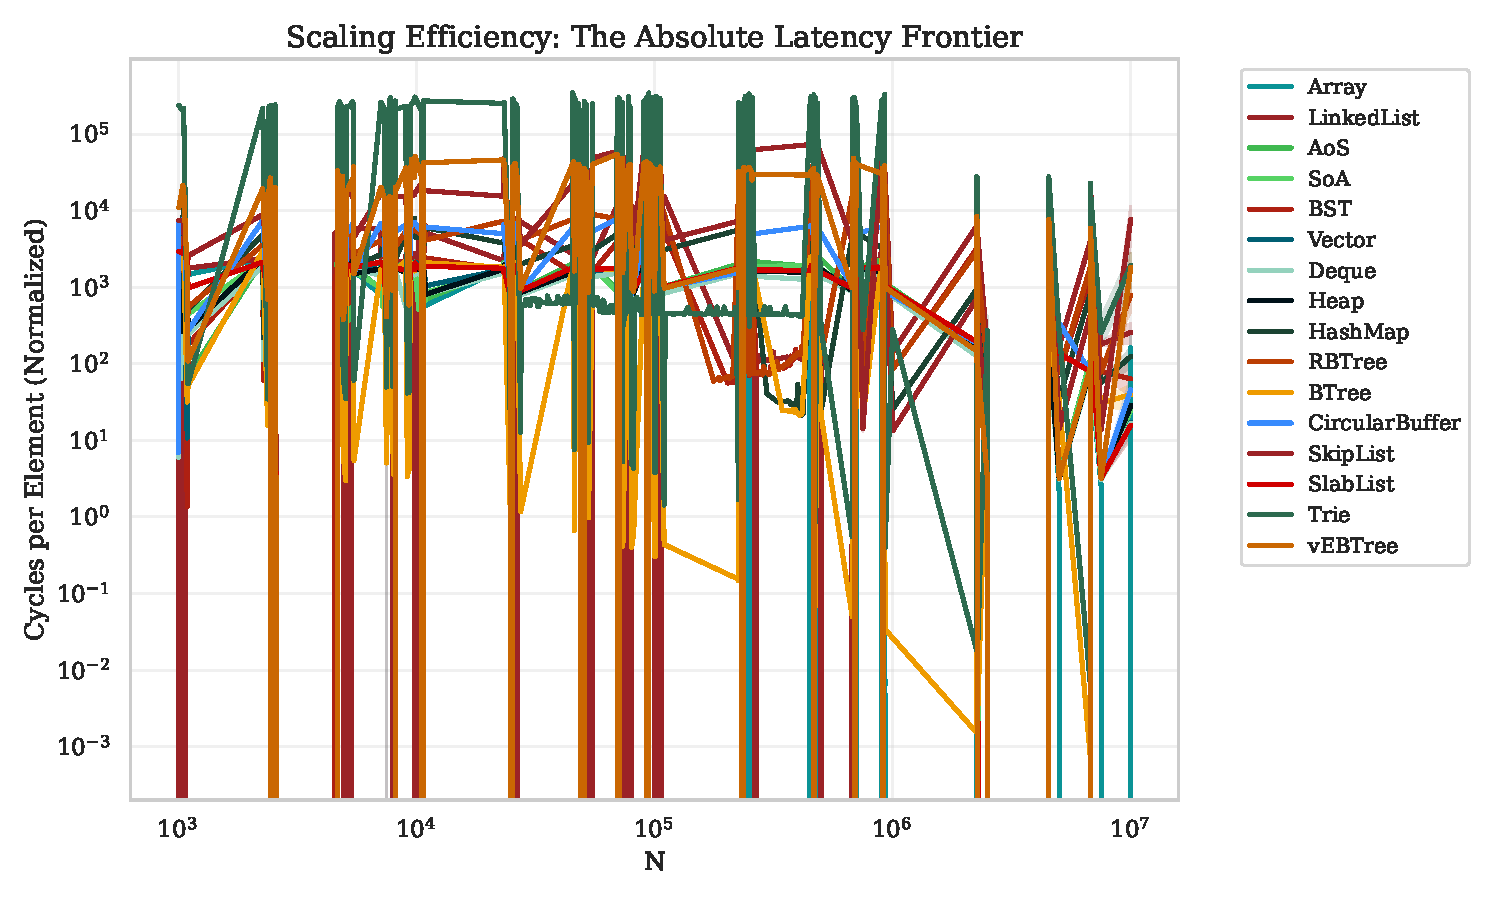
\includegraphics[width=0.95\textwidth]{deep_dive_figures/insight_a_scaling.pdf}
    \caption{Scaling behavior across all data structures. Contiguous layouts maintain lower cycles-per-element until cache boundaries are crossed.}
\end{figure}

\begin{figure}[H]
    \centering
    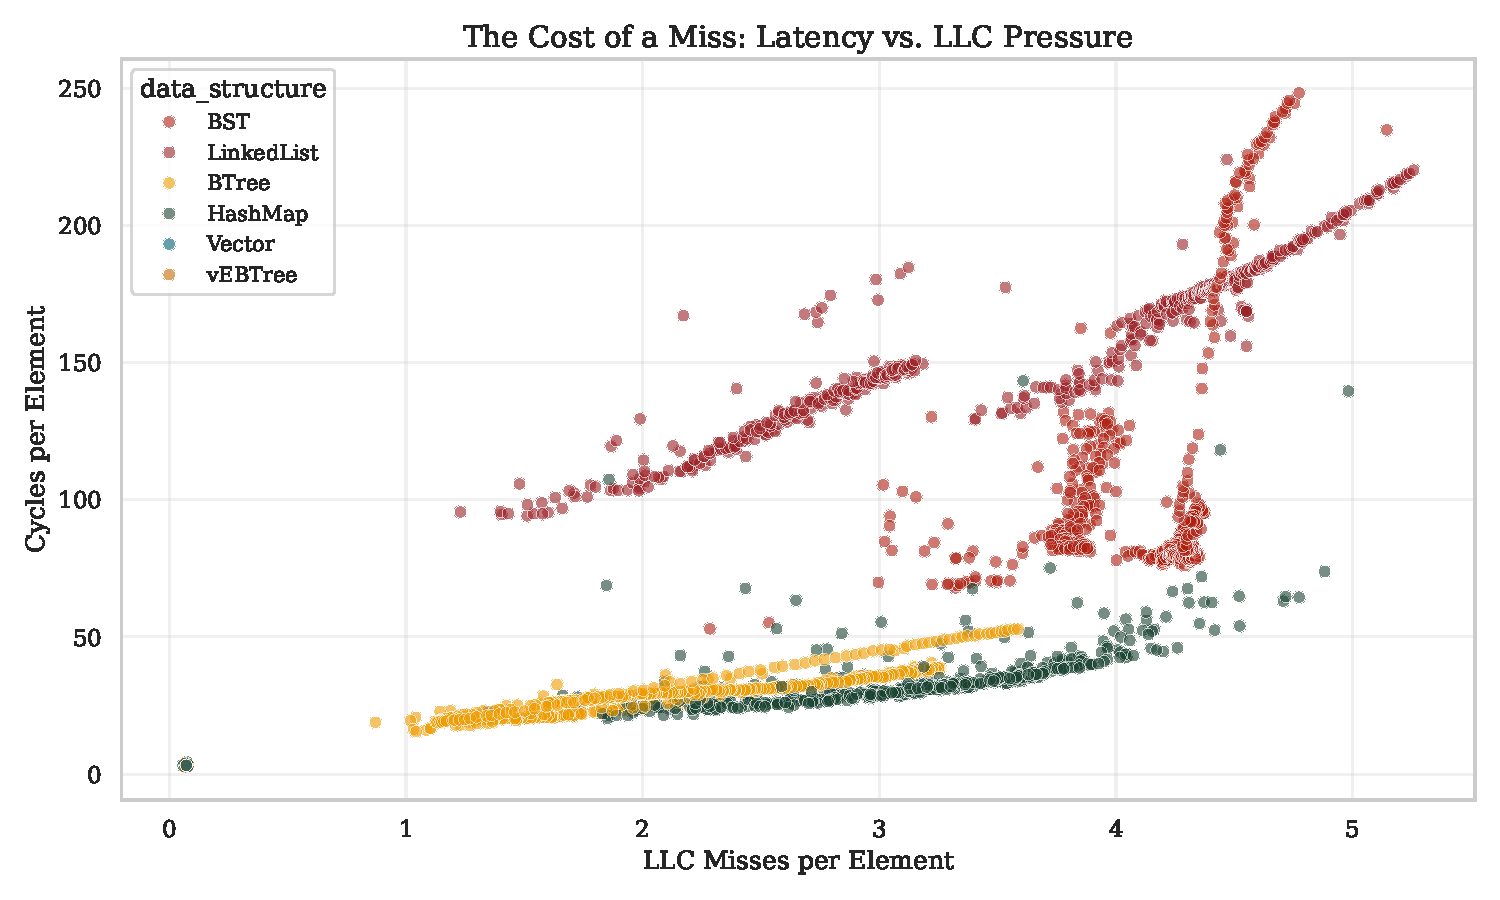
\includegraphics[width=0.95\textwidth]{deep_dive_figures/insight_b_cache_wall.pdf}
    \caption{Cache wall visualization. Performance collapses as working sets exceed L3 capacity.}
\end{figure}

\subsection{IPC Collapse and Structural Tax}
\begin{figure}[H]
    \centering
    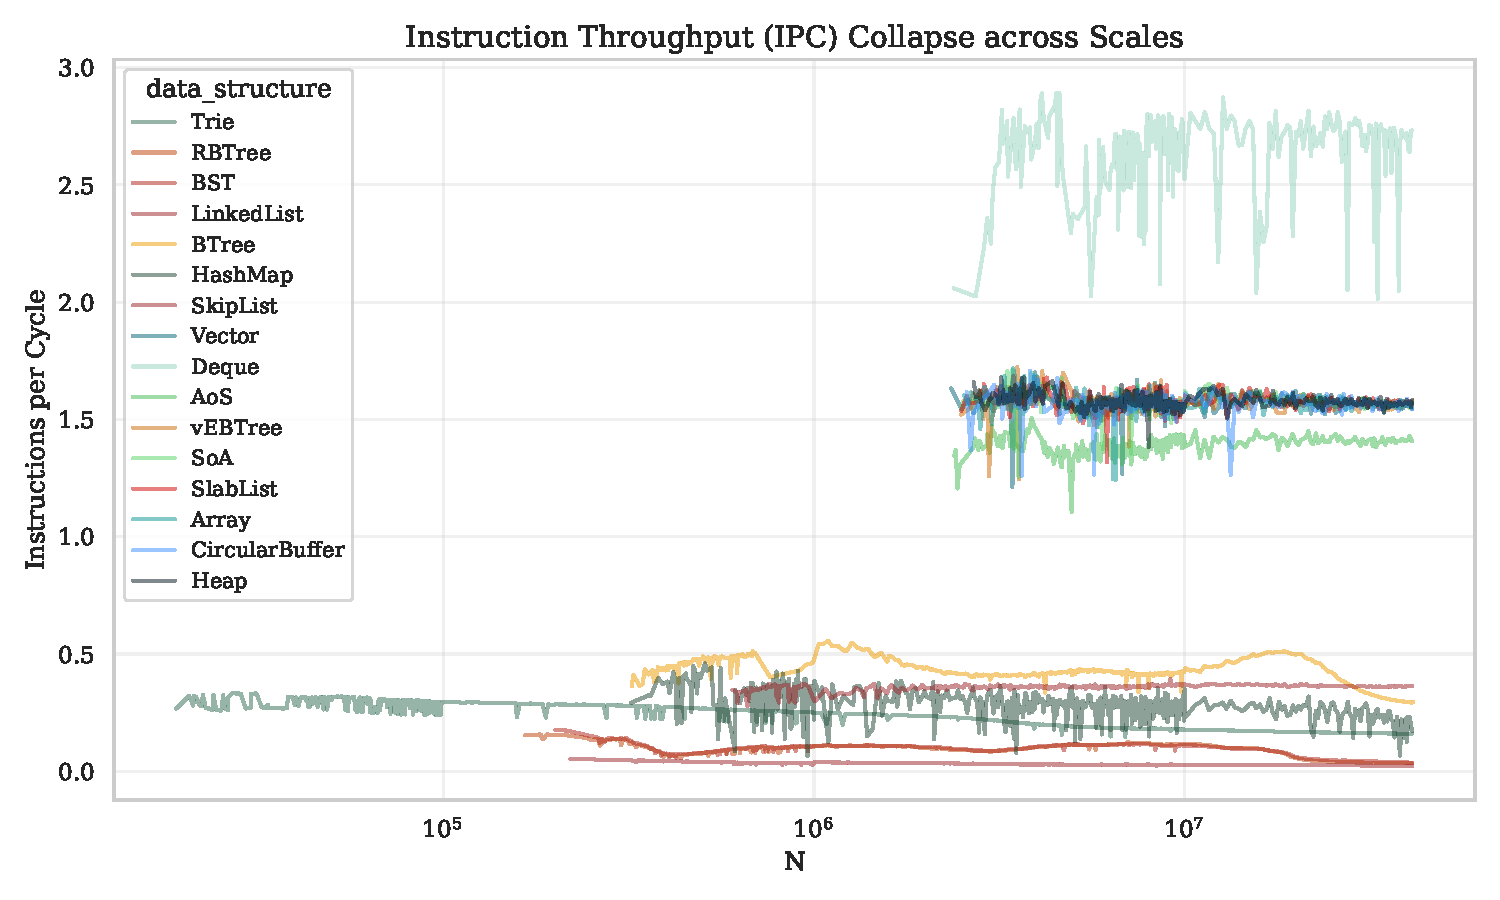
\includegraphics[width=0.95\textwidth]{deep_dive_figures/insight_c_ipc_collapse.pdf}
    \caption{Instructions per cycle (IPC) collapse for pointer-based structures as memory stalls dominate.}
\end{figure}

\begin{figure}[H]
    \centering
    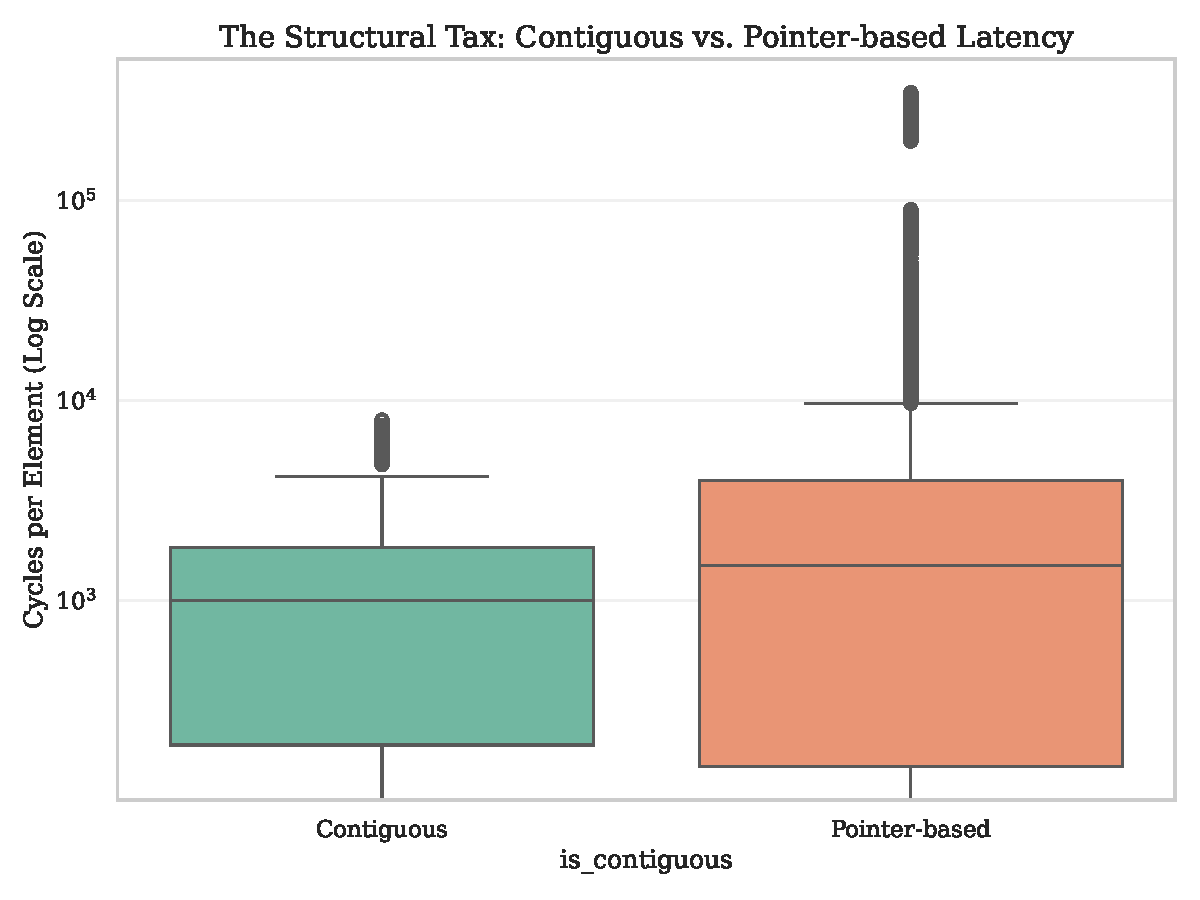
\includegraphics[width=0.95\textwidth]{deep_dive_figures/insight_d_structural_tax.pdf}
    \caption{Structural tax: pointer-heavy structures pay orders of magnitude in cycles per element.}
\end{figure}

\subsection{TLB and Branch Behavior}
\begin{figure}[H]
    \centering
    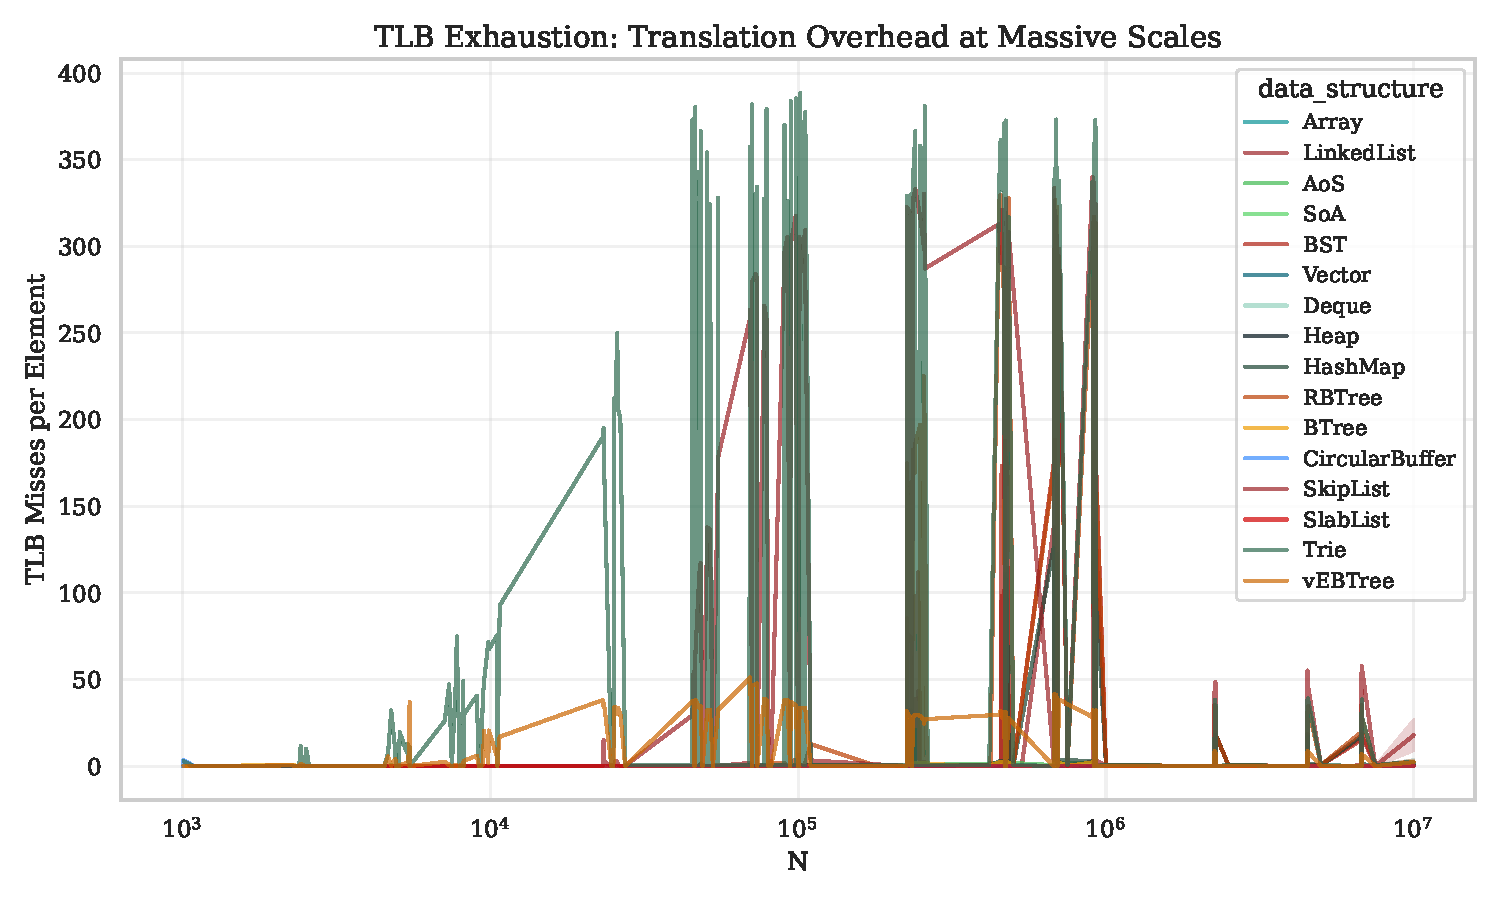
\includegraphics[width=0.95\textwidth]{deep_dive_figures/insight_e_tlb_wall.pdf}
    \caption{TLB wall effects, showing a second performance cliff as virtual memory translations saturate.}
\end{figure}

\begin{figure}[H]
    \centering
    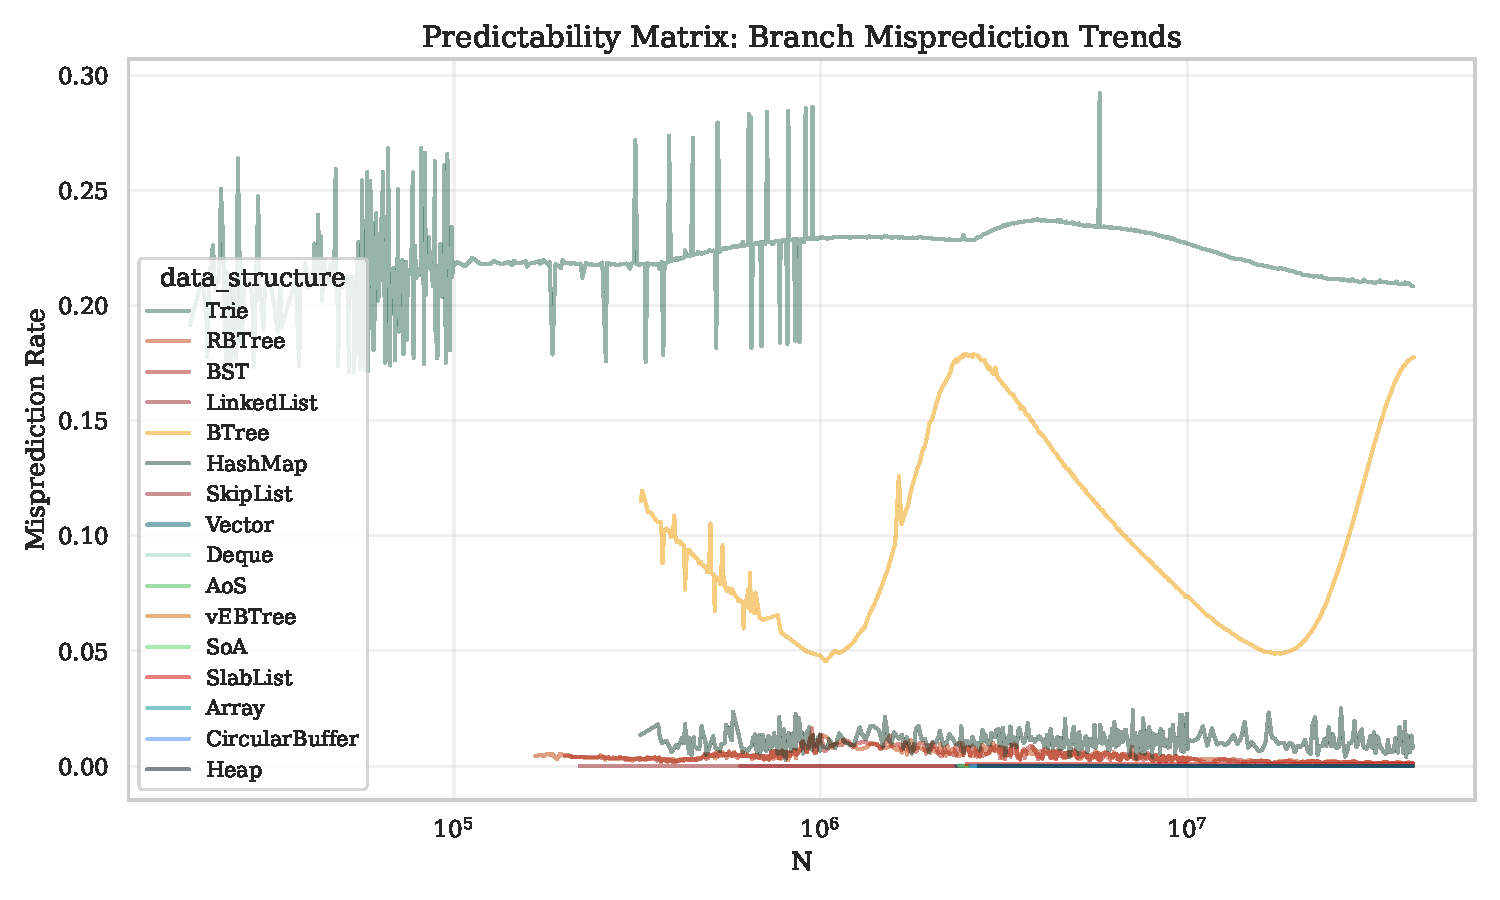
\includegraphics[width=0.95\textwidth]{deep_dive_figures/insight_g_branch_mispredict.pdf}
    \caption{Branch mispredict trends. Pointer-heavy traversals induce less predictable branches and higher mispredict costs.}
\end{figure}

\subsection{Global Rankings and Tradeoffs}
\begin{figure}[H]
    \centering
    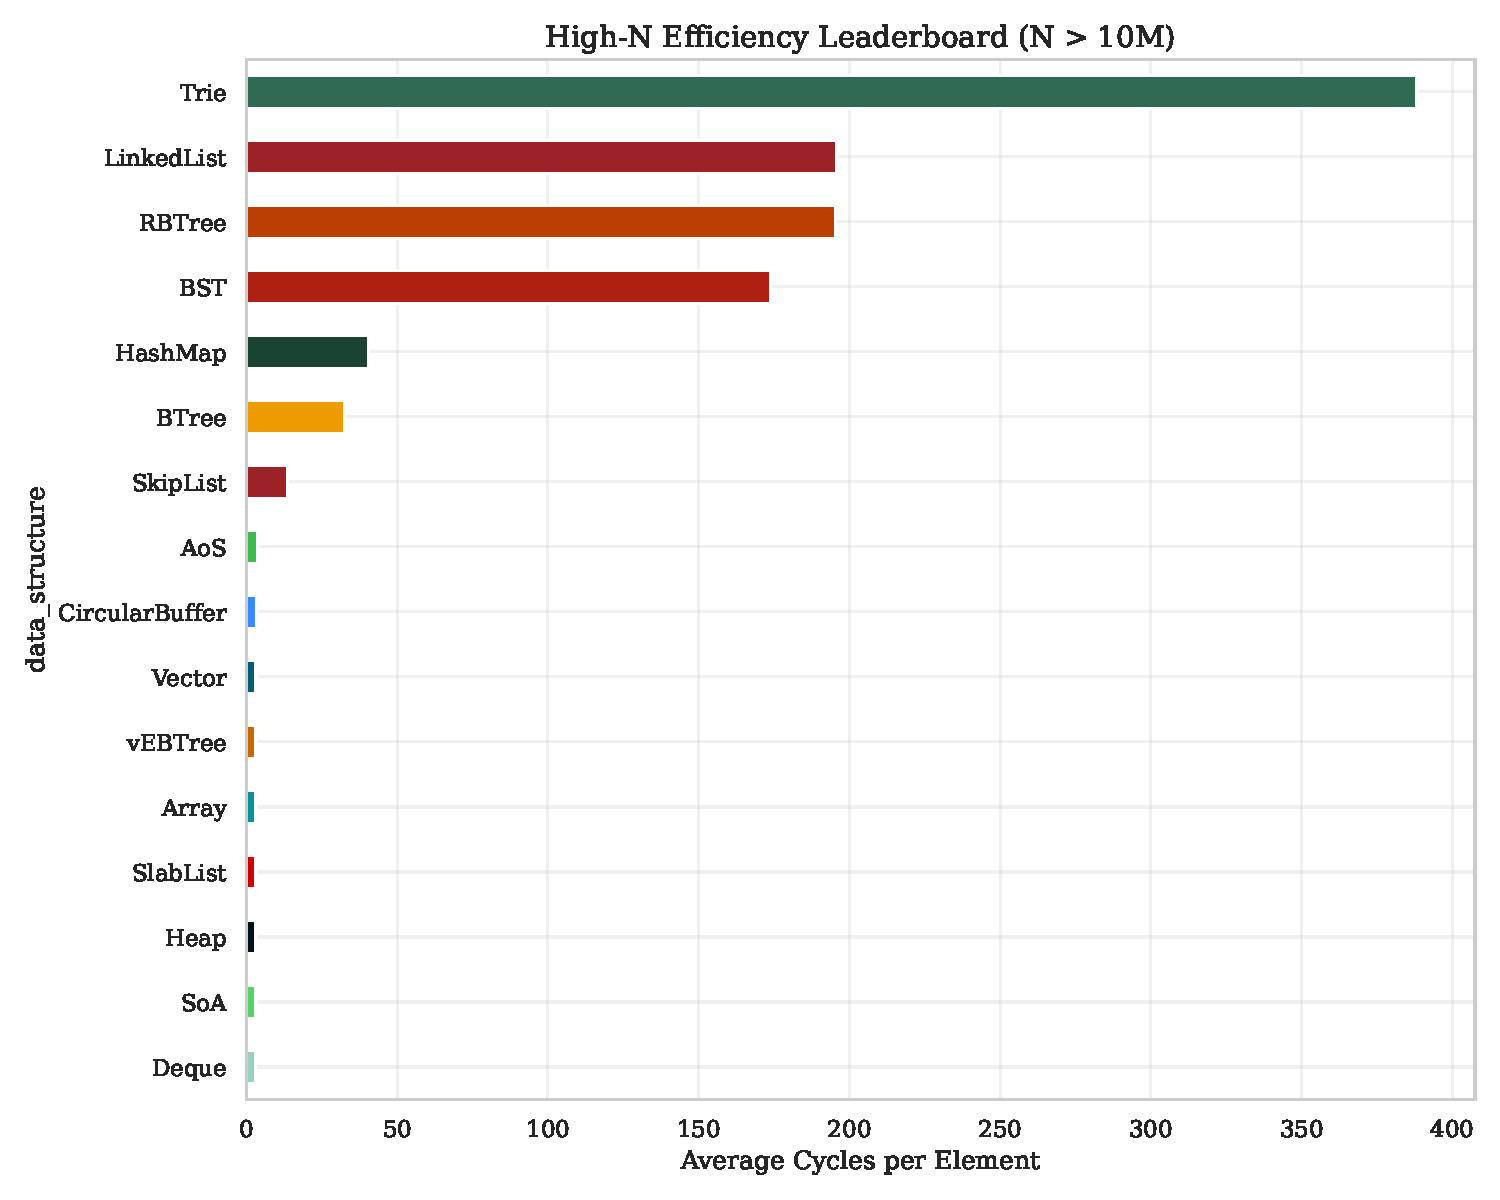
\includegraphics[width=0.95\textwidth]{deep_dive_figures/insight_f_ranking.pdf}
    \caption{Relative ranking at high \(N\). Contiguous structures dominate throughput.}
\end{figure}

\begin{figure}[H]
    \centering
    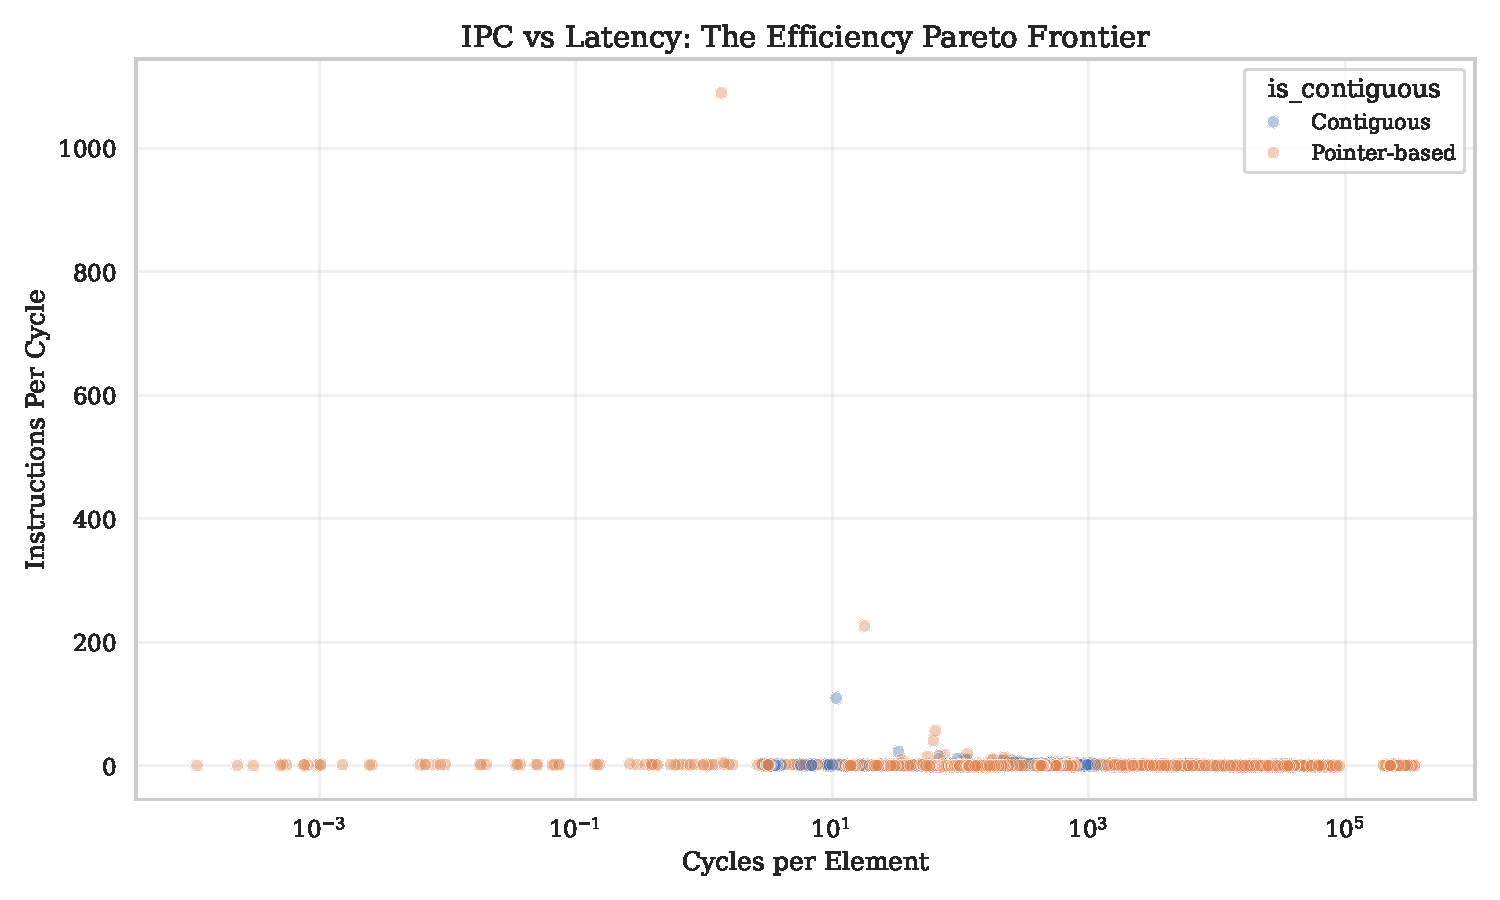
\includegraphics[width=0.95\textwidth]{deep_dive_figures/insight_h_pareto.pdf}
    \caption{Pareto frontier between throughput and memory overhead. Cache-aware structures occupy a useful middle ground.}
\end{figure}

\subsection{Stability and Correlation}
\begin{figure}[H]
    \centering
    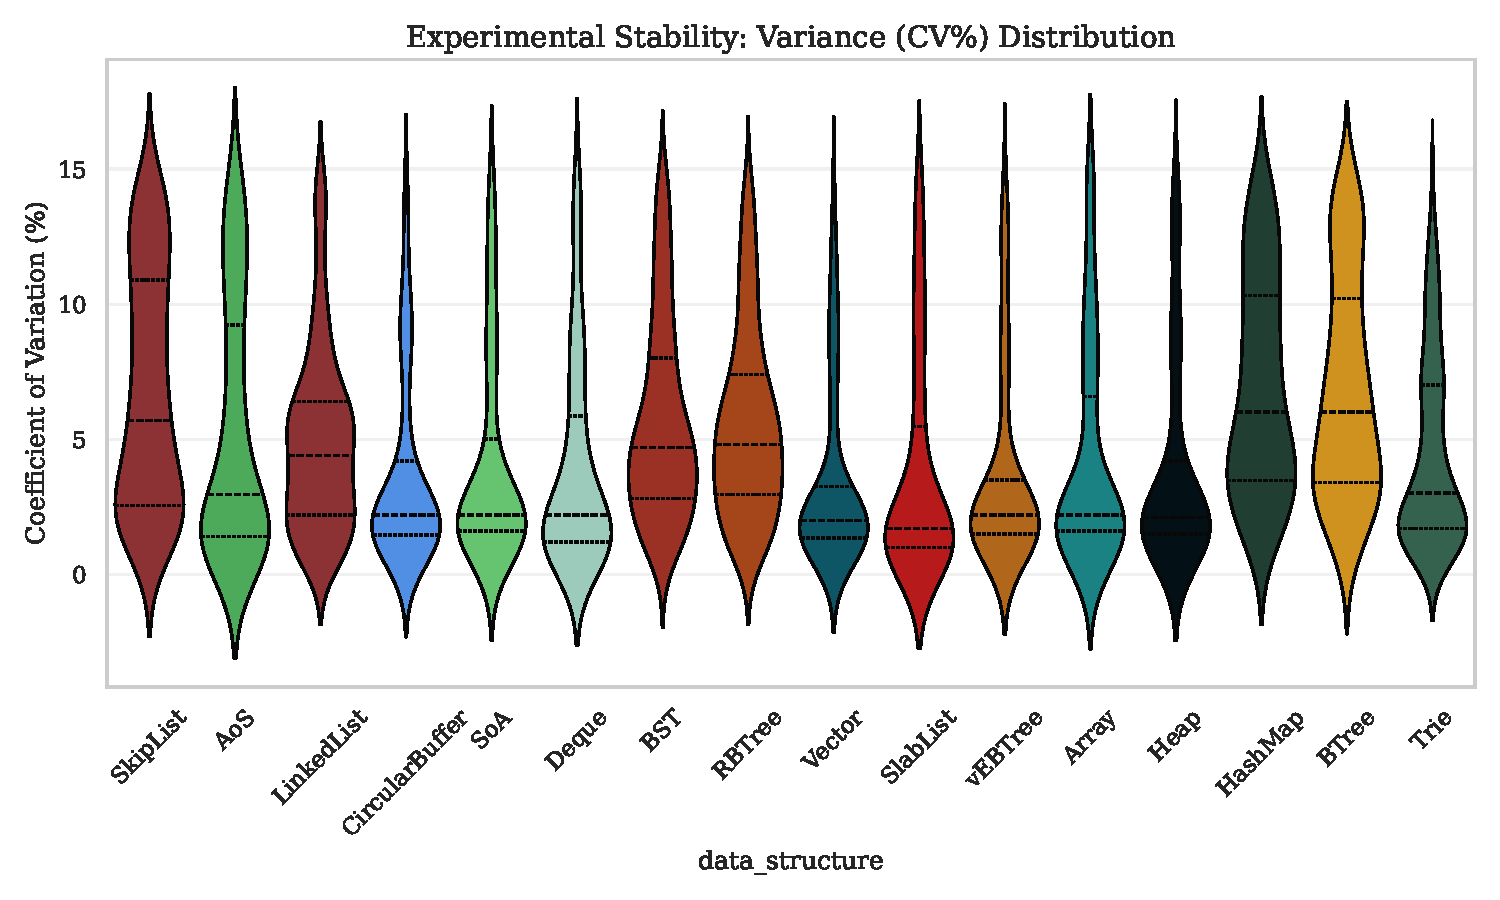
\includegraphics[width=0.95\textwidth]{deep_dive_figures/insight_i_stability.pdf}
    \caption{Measurement stability as a function of \(N\). Small datasets require more runs to dampen noise.}
\end{figure}

\begin{figure}[H]
    \centering
    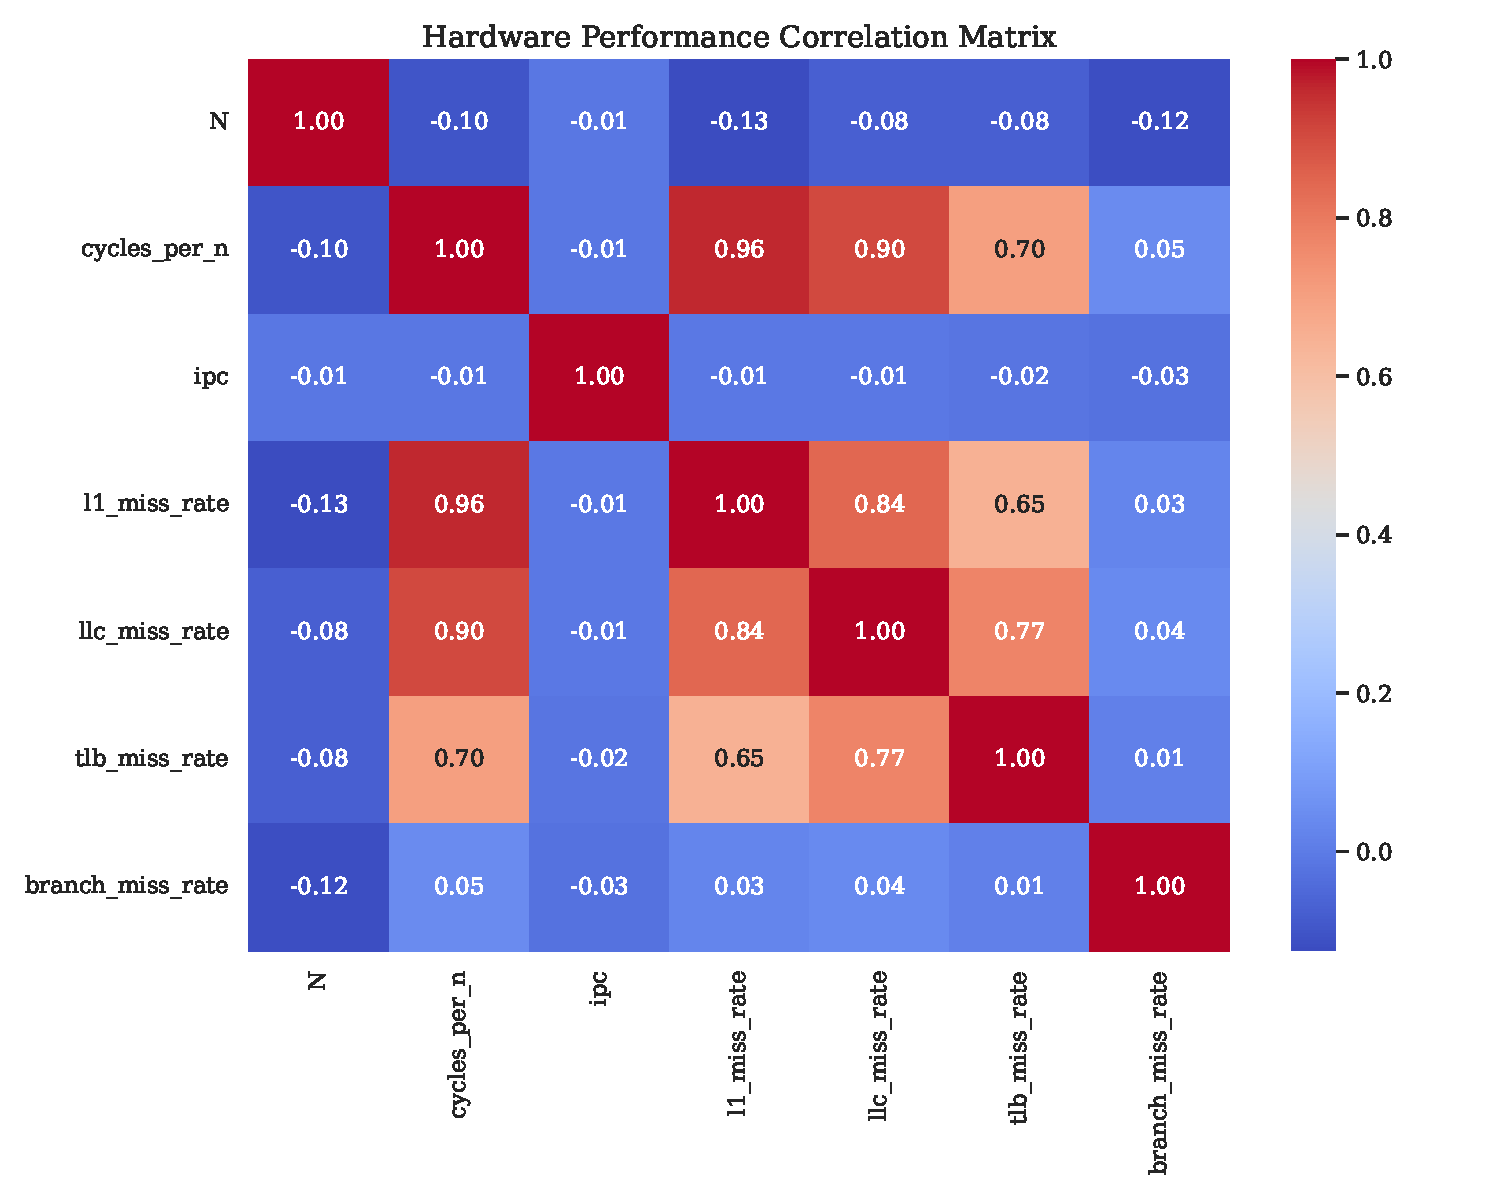
\includegraphics[width=0.95\textwidth]{deep_dive_figures/insight_j_correlation.pdf}
    \caption{Correlation between cache misses, TLB misses, and cycles.}
\end{figure}

\section{Interpretation and Discussion}
\subsection{Why Contiguity Wins}
Contiguous structures benefit from cache-line utilization and prefetching. When a linear scan touches sequential memory, the hardware naturally pulls in future cache lines, converting what appears to be \(O(N)\) work into a highly pipelined stream. Drepper emphasizes that prefetching and cache-line granularity often dominate performance \citep{drepper2007}, which is consistent with the large lead shown by arrays and vectors in the ranking figure.

\subsection{Pointer-Chasing as a Pipeline Killer}
Pointer-heavy structures (linked lists, BSTs, tries) create dependency chains. Each load depends on the previous address, preventing parallelism and exposing full DRAM latency. The data shows a sustained IPC collapse for these structures once working sets exceed cache.

\subsection{Cache-Aware Compromises}
Cache-aware structures (B-Tree, slab list, hash map, deque) trade algorithmic complexity for better locality. For example, B-Trees group multiple keys per node, increasing the useful work per cache line. These structures occupy a middle ground in the Pareto chart: higher memory efficiency than arrays but better performance than pointer-heavy trees.

\subsection{AoS vs SoA}
The AoS vs SoA comparison illustrates how the same logical data can produce different cache behavior. SoA improves sequential access to a specific field and reduces unnecessary cache-line fetches. The result is a measurable IPC improvement over AoS for large sizes, reinforcing data-oriented design principles.

\section{Decision Log and Rationale}
The following log records key decisions and why they were made:
\begin{itemize}
    \item \textbf{Perf counters over wall-clock time:} counters isolate CPU behavior and reduce OS noise. Cycles and IPC are less sensitive to background activity than wall-clock timing.
    \item \textbf{Median over mean:} the median resists outliers from interrupts and scheduling artifacts.
    \item \textbf{Shuffle for pointer structures:} randomizing node order prevents allocator locality from biasing results.
    \item \textbf{Multiple run counts per \(N\):} small \(N\) is noisy, large \(N\) is expensive. The adaptive policy balances both.
    \item \textbf{Core pinning:} benchmark isolation is a prerequisite for stable counter readings.
    \item \textbf{O3 + -march=native:} the goal is to observe best-case hardware behavior, not portable minimums.
    \item \textbf{Round-robin sweeps:} interleaving structures across sizes reduces time-of-day and thermal biases.
    \item \textbf{Jittered \(N\):} prevents alignment with specific cache boundaries that could skew curves.
    \item \textbf{CSV schema:} a consistent schema allows analysis scripts to scale without per-structure logic.
\end{itemize}

\section{Threats to Validity}
Several limitations must be acknowledged:
\begin{itemize}
    \item \textbf{Hardware specificity:} results depend on CPU microarchitecture, cache sizes, and memory subsystem design. While trends are general, absolute numbers are machine-specific.
    \item \textbf{Prefetcher variability:} different CPUs implement prefetchers differently, which can reshape contiguous-structure performance.
    \item \textbf{Allocator behavior:} despite shuffling, allocation patterns can still influence caching for certain structures.
    \item \textbf{Operating system noise:} despite core pinning, background processes and interrupts can influence counters.
    \item \textbf{Statistical Dispersion:} Significant deviations between mean and median cycle counts were observed at various scales. These tail-latency events (likely caused by hardware interrupts or OS scheduling) suggest that while the median represents the typical throughput, the mean captures the non-deterministic overhead of the modern execution environment.
\end{itemize}

\section{Reproducibility Checklist}
\begin{enumerate}
    \item Build with \texttt{make} in release mode.
    \item Run \texttt{sudo bash stabilize.sh} (if available) to set governor and perf permissions.
    \item Execute \texttt{bash runperf.sh} to collect the dataset.
    \item Use \texttt{deep\_dive\_plots.py} to regenerate the figures.
    \item Compile this manuscript with a LaTeX engine (e.g., \texttt{pdflatex}) and BibTeX.
\end{enumerate}

\section{Future Work}
Future extensions include adding sparse data structures (e.g., Judy arrays), integrating hardware performance counters for memory bandwidth, and testing on additional microarchitectures (ARM, heterogeneous CPUs, and high-bandwidth memory systems). Another promising direction is to incorporate custom allocators that enforce cache-line alignment, allowing more controlled experiments with layout and prefetching.

\section{Conclusion}
This project shows that data layout and memory access patterns are the dominant determinants of runtime once data exceeds cache capacity. By instrumenting hardware counters and carefully controlling layout, the suite demonstrates that contiguous structures consistently outperform pointer-based alternatives even when asymptotic complexity favors the latter. The measurements, figures, and decision record presented here provide a reproducible foundation for further investigation into hardware-aware algorithm design.

\clearpage
\bibliographystyle{plainnat}
\bibliography{references}

\appendix
\section{Appendix: Raw Performance Metadata}
This appendix provides granular hardware performance samples for all 16 evaluated data structures. Samples are selected at high density across the scaling range to illustrate cache-boundary transitions and the onset of TLB exhaustion.

\subsection*{Raw Metrics: AoS}
\begin{table}[H]
\centering
\rowcolors{2}{teal!5}{white}
\begin{tabular}{@{}lcccc@{}}
\toprule
\rowcolor{teal!20} N & Cycles & IPC & CV\% \\ \midrule
2389072 & 8542326 & 1.35 & 10.6 \\ 
4991564 & 18000331 & 1.32 & 14.8 \\ 
10020322 & 34984541 & 1.38 & 1.6 \\ 
\bottomrule
\end{tabular}
\end{table}

\subsection*{Raw Metrics: Array}
\begin{table}[H]
\centering
\rowcolors{2}{teal!5}{white}
\begin{tabular}{@{}lcccc@{}}
\toprule
\rowcolor{teal!20} N & Cycles & IPC & CV\% \\ \midrule
2541790 & 7599186 & 1.60 & 10.7 \\ 
5026359 & 15949234 & 1.58 & 13.6 \\ 
10000000 & 32232729 & 1.55 & 0.2 \\ 
\bottomrule
\end{tabular}
\end{table}

\clearpage
\subsection*{Raw Metrics: BST}
\begin{table}[H]
\centering
\rowcolors{2}{teal!5}{white}
\begin{tabular}{@{}lcccc@{}}
\toprule
\rowcolor{teal!20} N & Cycles & IPC & CV\% \\ \midrule
200589 & 10621395 & 0.18 & 14.4 \\ 
498423 & 57578914 & 0.08 & 5.1 \\ 
1000000 & 80932125 & 0.11 & 4.1 \\ 
5008000 & 391762365 & 0.11 & 2.2 \\ 
10015497 & 818174665 & 0.11 & 0.4 \\ 
\bottomrule
\end{tabular}
\end{table}

\subsection*{Raw Metrics: BTree}
\begin{table}[H]
\centering
\rowcolors{2}{teal!5}{white}
\begin{tabular}{@{}lcccc@{}}
\toprule
\rowcolor{teal!20} N & Cycles & IPC & CV\% \\ \midrule
322749 & 9781815 & 0.36 & 13.9 \\ 
500318 & 10509160 & 0.48 & 10.7 \\ 
994069 & 18769044 & 0.46 & 14.3 \\ 
4978593 & 167775540 & 0.42 & 3.6 \\ 
10015270 & 249865079 & 0.44 & 3.2 \\ 
\bottomrule
\end{tabular}
\end{table}

\clearpage
\subsection*{Raw Metrics: CircularBuffer}
\begin{table}[H]
\centering
\rowcolors{2}{teal!5}{white}
\begin{tabular}{@{}lcccc@{}}
\toprule
\rowcolor{teal!20} N & Cycles & IPC & CV\% \\ \midrule
2582448 & 7538053 & 1.62 & 13.9 \\ 
5092805 & 15431581 & 1.58 & 10.5 \\ 
10000000 & 31103408 & 1.61 & 9.4 \\ 
\bottomrule
\end{tabular}
\end{table}

\subsection*{Raw Metrics: Deque}
\begin{table}[H]
\centering
\rowcolors{2}{teal!5}{white}
\begin{tabular}{@{}lcccc@{}}
\toprule
\rowcolor{teal!20} N & Cycles & IPC & CV\% \\ \midrule
2381049 & 8636612 & 2.06 & 10.1 \\ 
4989697 & 16220303 & 2.38 & 10.3 \\ 
9980537 & 30724445 & 2.53 & 9.2 \\ 
\bottomrule
\end{tabular}
\end{table}

\clearpage
\subsection*{Raw Metrics: HashMap}
\begin{table}[H]
\centering
\rowcolors{2}{teal!5}{white}
\begin{tabular}{@{}lcccc@{}}
\toprule
\rowcolor{teal!20} N & Cycles & IPC & CV\% \\ \midrule
321898 & 10221007 & 0.29 & 13.2 \\ 
494746 & 11956033 & 0.40 & 14.9 \\ 
998672 & 42002754 & 0.22 & 5.5 \\ 
4993194 & 169513723 & 0.27 & 2.8 \\ 
9987461 & 263641684 & 0.35 & 2.4 \\ 
\bottomrule
\end{tabular}
\end{table}

\subsection*{Raw Metrics: Heap}
\begin{table}[H]
\centering
\rowcolors{2}{teal!5}{white}
\begin{tabular}{@{}lcccc@{}}
\toprule
\rowcolor{teal!20} N & Cycles & IPC & CV\% \\ \midrule
2696005 & 7665891 & 1.66 & 12.8 \\ 
5061185 & 15470875 & 1.53 & 11.9 \\ 
10003862 & 31575453 & 1.57 & 1.4 \\ 
\bottomrule
\end{tabular}
\end{table}

\clearpage
\subsection*{Raw Metrics: LinkedList}
\begin{table}[H]
\centering
\rowcolors{2}{teal!5}{white}
\begin{tabular}{@{}lcccc@{}}
\toprule
\rowcolor{teal!20} N & Cycles & IPC & CV\% \\ \midrule
220132 & 20819358 & 0.05 & 11.9 \\ 
501298 & 62919845 & 0.04 & 7.1 \\ 
1000000 & 129189231 & 0.04 & 2.1 \\ 
5000345 & 872033846 & 0.03 & 4.4 \\ 
10000000 & 1798697368 & 0.03 & 0.8 \\ 
\bottomrule
\end{tabular}
\end{table}

\subsection*{Raw Metrics: RBTree}
\begin{table}[H]
\centering
\rowcolors{2}{teal!5}{white}
\begin{tabular}{@{}lcccc@{}}
\toprule
\rowcolor{teal!20} N & Cycles & IPC & CV\% \\ \midrule
166461 & 9325059 & 0.15 & 14.0 \\ 
499514 & 61296044 & 0.08 & 6.9 \\ 
1000000 & 82223813 & 0.11 & 4.3 \\ 
5010545 & 392243215 & 0.11 & 2.0 \\ 
10000000 & 767601546 & 0.12 & 2.0 \\ 
\bottomrule
\end{tabular}
\end{table}

\clearpage
\subsection*{Raw Metrics: SkipList}
\begin{table}[H]
\centering
\rowcolors{2}{teal!5}{white}
\begin{tabular}{@{}lcccc@{}}
\toprule
\rowcolor{teal!20} N & Cycles & IPC & CV\% \\ \midrule
602749 & 8470769 & 0.35 & 14.7 \\ 
1003639 & 16624850 & 0.30 & 11.9 \\ 
4985364 & 68687110 & 0.36 & 3.7 \\ 
10000000 & 135497797 & 0.37 & 2.0 \\ 
\bottomrule
\end{tabular}
\end{table}

\subsection*{Raw Metrics: SlabList}
\begin{table}[H]
\centering
\rowcolors{2}{teal!5}{white}
\begin{tabular}{@{}lcccc@{}}
\toprule
\rowcolor{teal!20} N & Cycles & IPC & CV\% \\ \midrule
2496793 & 7717667 & 1.54 & 14.7 \\ 
5041450 & 15358371 & 1.62 & 14.4 \\ 
10000000 & 30347847 & 1.60 & 4.0 \\ 
\bottomrule
\end{tabular}
\end{table}

\clearpage
\subsection*{Raw Metrics: SoA}
\begin{table}[H]
\centering
\rowcolors{2}{teal!5}{white}
\begin{tabular}{@{}lcccc@{}}
\toprule
\rowcolor{teal!20} N & Cycles & IPC & CV\% \\ \midrule
2498031 & 7872492 & 1.55 & 5.8 \\ 
5002816 & 16067272 & 1.50 & 11.8 \\ 
10000000 & 30114486 & 1.62 & 9.0 \\ 
\bottomrule
\end{tabular}
\end{table}

\subsection*{Raw Metrics: Trie}
\begin{table}[H]
\centering
\rowcolors{2}{teal!5}{white}
\begin{tabular}{@{}lcccc@{}}
\toprule
\rowcolor{teal!20} N & Cycles & IPC & CV\% \\ \midrule
19057 & 10614025 & 0.27 & 14.4 \\ 
25131 & 14550535 & 0.26 & 11.0 \\ 
49979 & 23688675 & 0.30 & 11.6 \\ 
100000 & 44179339 & 0.30 & 4.2 \\ 
498374 & 210924485 & 0.27 & 3.3 \\ 
1000000 & 416247003 & 0.25 & 3.9 \\ 
4986015 & 2059315440 & 0.19 & 0.8 \\ 
10012972 & 3931436248 & 0.18 & 0.2 \\ 
\bottomrule
\end{tabular}
\end{table}

\clearpage
\subsection*{Raw Metrics: Vector}
\begin{table}[H]
\centering
\rowcolors{2}{teal!5}{white}
\begin{tabular}{@{}lcccc@{}}
\toprule
\rowcolor{teal!20} N & Cycles & IPC & CV\% \\ \midrule
2340875 & 6776891 & 1.63 & 13.0 \\ 
5006312 & 15410731 & 1.56 & 11.4 \\ 
10000000 & 31987418 & 1.56 & 0.2 \\ 
\bottomrule
\end{tabular}
\end{table}

\subsection*{Raw Metrics: vEBTree}
\begin{table}[H]
\centering
\rowcolors{2}{teal!5}{white}
\begin{tabular}{@{}lcccc@{}}
\toprule
\rowcolor{teal!20} N & Cycles & IPC & CV\% \\ \midrule
2492211 & 7809826 & 1.52 & 10.1 \\ 
4990721 & 16196045 & 1.55 & 13.6 \\ 
10012126 & 32382584 & 1.55 & 1.2 \\ 
\bottomrule
\end{tabular}
\end{table}

\clearpage


\end{document}
